\documentclass[14pt,titlepage]{extarticle}
\usepackage[pdftex,unicode,hidelinks]{hyperref}
\usepackage{ucs}
\usepackage[utf8x]{inputenc}
\usepackage[english,russian]{babel}
\usepackage{indentfirst}
\usepackage[usenames,dvipsnames]{color}
\usepackage{algorithm}
\usepackage{algorithmic}
\usepackage{amsmath}
\usepackage[pdftex]{graphicx}
\usepackage{multicol}

% TODO Change geometry: left=3cm,right=2cm !
\usepackage[left=2.5cm,right=2.5cm,top=2cm,bottom=2cm,bindingoffset=0cm]{geometry}
\linespread{1.3}

\usepackage{numprint}
\newcommand{\num}[1]{\numprint{#1}}
  \npthousandsep{\,}
  \npthousandthpartsep{}
  \npdecimalsign{,}

\usepackage{tikz}
\usetikzlibrary{arrows,shapes}

\bibliographystyle{gost780u}

%\setcounter{tocdepth}{2} % глубина оглавления

\floatname{algorithm}{Пример}
\newcommand{\algorithmictitle}[1]{\hspace{8mm}\textbf{#1}}
\renewcommand{\algorithmicrequire}{\textbf{Дано:}}
\renewcommand{\algorithmiccomment}[1]{// #1}
\newcommand{\NEW}{\textbf{new }}
\newcommand{\NEWi}[1]{\textbf{new}_{#1}\textbf{ }}
\newcommand{\NULL}{\textbf{null }}
\newcommand{\BOOLTRUE}{\textbf{true }}
\newcommand{\FUNCTION}{\textbf{function }}

\newcommand{\Pts}[1]{\textrm{Pts}(#1)}
\newcommand{\VPts}[1]{\textrm{VarPts}(#1)}
\newcommand{\OFPts}[2]{\textrm{ObjectFieldPts}(#1, #2)}
\newcommand{\SharedOFPts}[2]{\textrm{SharedObjectFieldPts}(#1, #2)}
\newcommand{\Filter}[2]{\textrm{Filter}_{#1}(#2)}
\newcommand{\IsAssignable}[2]{\textrm{IsAssignable}(#1, #2)}
\newcommand{\cupe}{\,\cup\!\!=}

\let\oldphi\phi
\renewcommand{\phi}{\ensuremath{\oldphi}}

%\newcommand{\remark}[1]{}
%\newcommand{\todo}[1]{}
%\newcommand{\todocite}{}
\newcommand{\remark}[1]{\textcolor{Green}{#1}}
\newcommand{\todo}[1]{\textcolor{red}{\eng{TODO}: #1}}
\newcommand{\todocite}{[\todo{cite}]}

\newcommand{\eng}[1]{{\English#1}}

\addto\captionsrussian{
  \let\oldrefname\refname
  \renewcommand\refname{\addcontentsline{toc}{section}{\oldrefname}\oldrefname}
}

\let\oldsection\section
\renewcommand{\section}{\newpage\oldsection}

\newcommand{\sectionwithoutnumber}[1]{
  \section*{#1}
  \addcontentsline{toc}{section}{#1}
}

\title{
  Анализ указателей и синонимов для многопоточных программ
}
\author{
  Владимир Парфиненко
}

\begin{document}

  \thispagestyle{empty}
  \begin{center}

    Министерство образования и науки\\
    Российской Федерации

    \vspace{0.7cm}

    Государственное образовательное учреждение\\
    высшего профессионального образования\\
    «Новосибирский государственный университет» (НГУ)

    \vspace{0.7cm}

    Физический факультет

    \vspace{0.2cm}

    Кафедра автоматизации физико-технических исследований

    \vspace{1.2cm}

    Квалификационная работа на соискание\\
    степени бакалавра

    \vspace{0.2cm}

    Парфиненко Владимир Владимирович

    \vspace{1.5cm}

    \textbf{АНАЛИЗ УКАЗАТЕЛЕЙ И СИНОНИМОВ\\ ДЛЯ МНОГОПОТОЧНЫХ ПРОГРАММ}

    \vspace{2.5cm}

    \begin{flushright}

      Научный руководитель

      м.\,н.\,с.~ИСИ~СО~РАН, Павлов\,П.\,Е.

    \end{flushright}

    \vspace {4cm}

    Новосибирск~--- 2011~год
  \end{center}

  \tableofcontents

  \sectionwithoutnumber{Введение}

    Средства оптимизации программ нужны для получения высокой
    скорости исполнения программ или улучшения других характеристик программы.

    Под оптимизацией программ понимается преобразование программы в
    семантически эквивалентную, но более эффективную относительно некоторого
    заданного критерия.
    Преобразование программы $A$ в программу $B$ эквивалентно (или корректно),
    если из того, что программа $A$ выполнима на некотором наборе данных,
    следует, что и $B$ также выполнима на этом наборе и дает тот же результат,
    что и $A$.
    В общем случае задача проверки эквивалентности двух программ неразрешима,
    и не существует алгоритма, который по данной программе находил бы
    эквивалентную ей и оптимальную относительно заданного критерия
    \cite{kasjanov_translators}.

    Тем не менее существует набор известных оптимизирующих преобразований,
    таких, что корректность каждого из них гарантирует корректность их
    последовательного применения.
    И чтобы конкретное преобразование данной программы было корректным,
    необходимо выполнение некоторых условий. Например, чтобы иметь
    возможность убрать генерацию некоторой части программы, нужно быть
    увереным, что управление никогда не попадет в эту часть программы.
    Для получения подобной информации используют результаты статического
    анализа. Анализируя код программы, делаются выводы о тех или иных свойствах
    программы, необходимых для проведения преобразования.

    Статический анализ применяется не только для проверки
    корректности преобразований, но и в инструментах статического анализа
    кода программ, которые могут находить потенциальные ошибки и определять
    другие свойства программы без ее непосредственного исполнения.

    Существует множество видов статического анализа, в данной работе
    рассматриваются анализ указателей и анализ синонимов.

  \section{Анализ указателей}

    Анализ указателей~--- это один из видов статического анализа, который
    позволяет определить, на какие объекты в памяти могут указывать выражения
    ссылочного типа в программе (такие объекты называются целями выражения
    ссылочного типа). Анализ синонимов похож на анализ указателей: его целью
    является определение, могут ли два разных выражения ссылаться на одно и
    то же место в памяти (такие выражения называют синонимами)
    \cite{andersen}.

    Существует множество алгоритмов анализа указателей и синонимов,
    \todo{Паше что-то не понравилось:}
    одним из них является алгоритм анализа, основанный на типах
    (\eng{Type-Based Alias Analysis}) \cite{diwan_tbaa},
    применимый для языков со строгой типизацией.
    В языках со строгой типизацией любая ссылочная переменная формального типа
    $T$ может указывать на объекты типа $T$ или его наследников
    (подробнее про строгую систему типов в разделе \ref{section:type_system}).
    Простейшая реализация алгоритма, основанного на типах, дает следующий
    результат: независимо от контекста и потоков данных в программе целями
    выражения ссылочного типа являются все объекты совместимые по присваиванию
    с этим выражением.
    Такой алгоритм работает быстро, но обладает сравнительно низкой точностью.

    Для сравнения точности алгоритмов анализа указателей необходимо ввести
    некую меру точности. В качестве простой меры точности алгоритма обычно
    используется усредненное количество синонимов для переменных ссылочного
    типа, появляющихся в программе \cite{hind_pointer_analysis_not_solved_yet}
    \todo{сказать про другие меры?}.
    Понятно, что для «идеального» алгоритма анализа это число будет
    минимальным, а для самого консервативного алгоритма максимальным.

    \subsection{Классификация алгоритмов анализа указателей}
    \label{section:analysis_classification}

      Далее рассмотрим более точные алгоритмы анализа, учитывающие следующие
      свойства анализируемой программы:
      \begin{enumerate}
        \item потоки данных внутри функции;
        \item поток управления;
        \item потоки данных между функциями.
      \end{enumerate}

      Во-первых, алгоритмы анализа указателей могут учитывать потоки данных в
      программе.
      Например, если существует только одно присваивание вида $v = \NEW T()$,
      то можно гарантировать, что переменная $v$ может указывать только на
      объект, созданный этим оператором \eng{new}.
      С присваиванием вида $v_1 = v_2$ ситуация сложнее. Рассмотрим пример
      \ref{code:data_flow}.
      \begin{algorithm}
        \caption{Сравнение \eng{subset-based} и \eng{equality-based} алгоритмов}
        \label{code:data_flow}
        \begin{algorithmic}[1]
          \STATE $b$ = \NEW T()
          \STATE $c$ = \NEW T()
          \STATE $a$ = $b$
          \STATE $a$ = $c$
        \end{algorithmic}
      \end{algorithm}

      Цели указателя, то есть множество объектов, на которые может указывать
      переменная $p$ (или любое другое выражение ссылочного типа), для удобства
      обозначим как $Pts(p)$ (англ. \eng{points-to set}).
      Учитывая строки 1 и 2, для переменных $b$ и $c$ мы можем точно определить
      множество объектов, на которые они указывают:
      \[Pts(b) = \{O_1\}, Pts(c) = \{O_2\},\] где $O_1$ и $O_2$~--- уникальные
      объекты в куче, соответствующие операторам \eng{new} в строках 1 и 2.
      То есть мы учли поток данных от оператора \eng{new}, создавшего новый
      объект, в переменную.

      Интерпретировать присваивание $a = b$ можно двумя способами,
      и алгоритмы анализа разбиваются на два типа по этому признаку:
      \begin{itemize}
        \item алгоритмы первого типа накладывают ограничение
              $Pts(a) \supset Pts(b)$ (\eng{subset-based} алгоритмы)
              \cite{rayside_overview},
        \item алгоритмы второго типа накладывают ограничение
              $Pts(a) = Pts(b)$ (\eng{equality-based} алгоритмы)
              \cite{rayside_overview}.
      \end{itemize}
      Первый тип алгоритмов более точен, в то время как второй быстрее
      \cite{steensgaard}. Возвращаясь к нашему примеру, \eng{subset-based}
      алгоритм получит, что
      \[Pts(a) = \{O_1, O_2\}, Pts(b) = \{O_1\}, Pts(c) = \{O_2\},\]
      а \eng{equality-based}
      \[Pts(a) = Pts(b) = Pts(c) = \{O_1, O_2\}.\]

      Во-вторых, для повышения точности алгоритм может учитывать поток
      управления в программе.
      Рассмотрим пример \ref{code:control_flow}.
      \begin{algorithm}
        \caption{Сравнение чувствительного и нечувствительного к потоку
                 управления алгоритмов}
        \label{code:control_flow}
        \begin{algorithmic}[1]
          \STATE $a$ = \NEW T()
          \STATE $b$ = \NEW T()
          \STATE $c$ = \NEW T()
          \STATE $a$ = $b$
          \STATE $b$ = $c$
          \STATE $c$ = $a$
        \end{algorithmic}
      \end{algorithm}

      Нечувствительный к потоку управления алгоритм анализа воспринимает
      программу не как последовательность операций (\todo{Паше что-то не
      понравилось}), а как их неупорядоченный набор.
      Для указанного примера такой алгоритм получит следующее
      \[Pts(a) = Pts(b) = Pts(c) = \{O_a, O_b, O_c\}.\]
      Этот результат не является особо точным, но зато он верен
      для любой точки программы.

      Чувствительный к потоку управления алгоритм получит следующие данные
      после 3-ей строки
      \[\textrm{строка 3}:
          Pts(a) = \{O_a\}, Pts(b) = \{O_b\}, Pts(c) = \{O_c\}.\]
      Далее, при анализе 4-ой строки, присваивание будет интерпретированно как
      строгое присваивание (подробнее в разделе
      \ref{section:flow_sensetive_analysis}), и алгоритм получит
      результат, что $Pts(a) = \{O_b\}$. То есть присваивание нового значения
      в переменную уничтожило информацию о том, что $a$ может указывать на $O_a$.
      Продолжая подобные рассуждения до последней строки, получаются следующие
      результаты:
      \[\textrm{строка 6}:
          Pts(a) = \{O_b\}, Pts(b) = \{O_c\}, Pts(c) = \{O_b\}.\]
      Хотя такой алгоритм дает более точный результат, приходится хранить
      информацию о целях каждого указателя для каждой операции отдельно,
      что значительно увеличивает суммарный объем памяти, занимаемый
      информацией о целях указателей.

      В-третьих, алгоритм анализа может учитывать потоки данных между отдельными
      функциями и процедурами
      (\todo{Паша предложил окончить предложение здесь})
      для повышения точности анализа.
      Рассмотрим пример \ref{code:interprocedural}.
      \begin{algorithm}
        \caption{Демонстрация работы межпроцедурного алгоритма}
        \label{code:interprocedural}
        \begin{algorithmic}[1]
          \STATE \FUNCTION foo($x$, $y$) \{
          \RETURN $x$
          \STATE \}
          \STATE
          \STATE $b$ = \NEW T()
          \STATE $c$ = \NEW T()
          \STATE $a$ = foo($b$, $c$)
        \end{algorithmic}
      \end{algorithm}

      Наша задача понять, чему равно $Pts(a)$.
      Алгоритмы анализа можно разделить на две категории, в зависимости от
      того, как они обрабатывают вызовы функций:
      \begin{itemize}
        \item межпроцедурные алгоритмы анализа могут сначала проанализировать
              тело вызываемой функции, и затем учесть результат при обработке
              вызова,
        \item внутрипроцедурные алгоритмы рассматривают вызов функции в
              наиболее консервативном предположении: может быть возвращен либо
              один из параметров, либо один из глобальных объектов.
      \end{itemize}
      Понятно, что первый тип алгоритмов дает более точные результаты,
      а второй потребляет меньше памяти и работает быстрее
      \cite[с.~117]{andersen}.
      В нашем примере межпроцедурный алгоритм анализа, проанализировав функцию
      foo, запоминает, что для нее выполнено следующее условие на возвращаемое
      значение
      \[Pts(retval) = Pts(x),\]
      и тогда может сделать вывод, что \[Pts(a) = Pts(b) = \{O_1\}.\]
      В такой же ситуации внутрипроцедурный алгоритм анализа обязан сделать
      консервативное предположение
      \[Pts(a) = Pts(b) \cup Pts(c) = \{O_1, O_2\}.\]

  \section{Описание предметной области}

    \subsection{Место алгоритмов анализа в компиляторе}

      Рассмотрим общую архитектуру оптимизирующего статического компилятора.

      \begin{figure}[!htb]
        \center{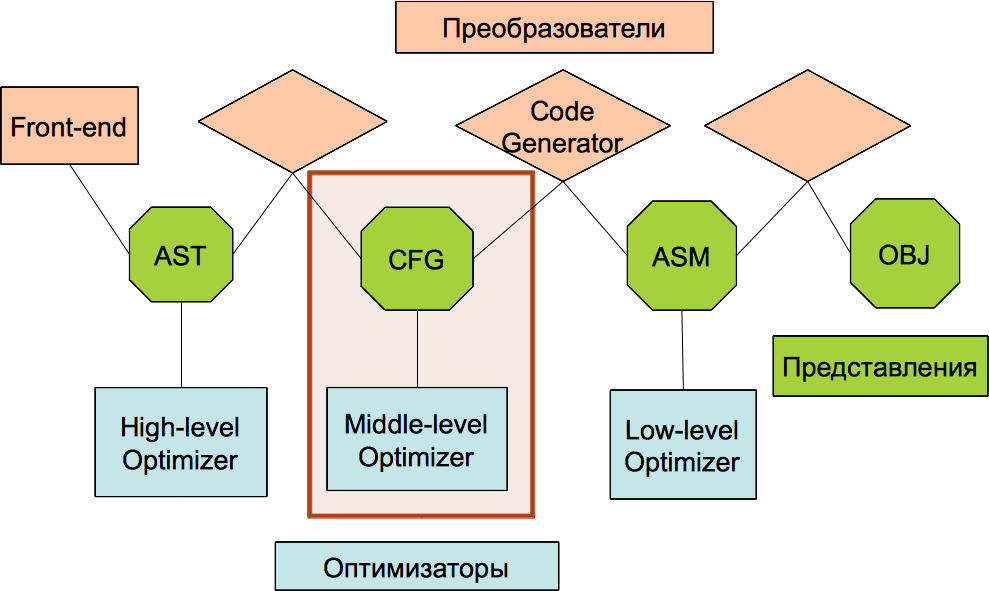
\includegraphics[width=140mm]{arch}}
        \caption{Архитектура оптимизирующего статического компилятора
                 \todo{перевести на tikz}}
        \label{fig:arch}
      \end{figure}

      Такой компилятор представляет из себя конвейер (см. рис. \ref{fig:arch}):
      на входе он получает исходный код программы, на выходе отдает код целевой
      машины.
      Также существуют промежуточные представления, пригодные для работы
      оптимизаторов и необходимых им алгоритмов анализа.

      Для перевода программы из одного представления в другое существуют
      преобразователи.
      Самый первый преобразователь переводит исходный код программы
      или байт-код программы (в случае Java)
      во внутреннее представление, с которым удобно работать другим
      компонентам компилятора.
      Последний преобразователь выполняет перевод в самое низкоуровневое
      представление, содержащее данные и код, пригодный для исполнения
      на целевой машине.

      Оптимизации проводятся на одном из внутренних представлений, они
      модифицируют его с целью повышения эффективности исполнения программы
      относительно заданного критерия. Однако, эти преобразования должны быть
      корректными. Информацию о том, возможно ли проведение данного
      преобразования, можно получать от анализаторов, вспомогательных
      компонент, которые проводят статический анализ программы и могут
      предоставлять ту или иную информацию о ее свойствах.

      \begin{figure}[!htb]
        \centering

        \tikzstyle{optimizer} = [rectangle, draw, thin, fill=blue!10,
                            minimum height=2em, rounded corners=1mm,
                            text width=3cm, text centered]
        \tikzstyle{analyzer} =  [rectangle, draw, thin, fill=blue!20,
                            minimum height=2em, rounded corners=1mm,
                            text width=3cm, text centered]

        \begin{tikzpicture}[node distance=5cm, auto,>=latex', thick]
          \path[->] node[optimizer] (o1) {Common Subexpression Elimination}
                    node[optimizer, right of=o1] (o2) {Another Optimization}
                    node[optimizer, right of=o2] (o3) {Loop Invariant Code Motion};
          \path[->] node[analyzer, below of=o1] (a1) {Another Analysis}
                    node[analyzer, below of=o2, line width=1] (a2) {Alias Analysis}
                    node[analyzer, below of=o3] (a3) {Another Analysis}
                    (o1) edge (a1) edge (a2)
                    (o2) edge (a2) edge (a3)
                    (o3) edge (a2);
        \end{tikzpicture}
      \end{figure}

      Рассмотрим оптимизацию выноса инвариантов цикла (англ.
      \eng{loop invariant code motion}) на примере \ref{code:licm}.
      Для выноса какого-либо выражения из цикла, требуется убедиться, что оно
      не будет изменяться (является инвариантом цикла).
      В данном примере, кандидатом на вынесение из цикла является выражение
      $x.field$. Оптимизатору необходимо убедиться, что поле объекта, на
      который ссылается переменная $x$ не изменяется при выполнении других
      операций в теле цикла. В данном примере оптимизатору необходимо знать,
      могут ли переменные $x$ и $y$ быть синонимами. Если могут, то
      проводить преобразование нельзя, так как запись в $y.field$ может
      изменить значение $x.field$. Если же переменные точно не являются
      синонимами, то вынос $x.field$ из цикла является корректным
      преобразованием.

      \begin{algorithm}
        \caption{Вынесение инвариантов цикла}
        \label{code:licm}
        \begin{multicols*}{2}
          \algorithmictitle{Исходный код}
          \begin{algorithmic}[1]
            \FOR{$i = 1$ to \textbf{length}($a$)}
            \STATE $y.field = func(i)$
            \STATE $a[i] = x.field$
            \ENDFOR
          \end{algorithmic}
          \columnbreak
          \algorithmictitle{Преобразованный код}
          \begin{algorithmic}[1]
            \STATE $temp = x.field$
            \FOR{$i = 1$ to \textbf{length}($a$)}
            \STATE $y.field = func(i)$
            \STATE $a[i] = temp$
            \ENDFOR
          \end{algorithmic}
        \end{multicols*}
      \end{algorithm}

      Анализ синонимов, описанный в работе, позволяет отвечать на
      вопрос оптимизатора: «А могут ли две переменные ссылочного типа быть
      синонимами?»

    \subsection{Анализ многопоточных программ}
      \label{section:intro_to_multithreading}

      Компьютеры, в которых несколько процессоров взаимодействуют с
      использованием разделяемой памяти, разрабатываются с 1960-х годов, а
      сейчас они уже распространены повсеместно.

      С одной стороны, изначально доступ к общей памяти был строго
      последовательным для всех потоков, исполнявшихся на разных процессорах.
      Это приводило к тому, что два последовательных чтения в одном потоке из
      одного и того же места памяти могли давать разные результаты, так как в
      параллельном потоке могла быть совершена запись в эту же самую память в
      момент времени между последовательными чтениями в первом потоке.

      С другой стороны, со временем появились весьма изощренные техники
      повышения производительности работы с общей памятью: многоуровневые кэши,
      внеочередное исполнение и другие.
      Это приводит к тому, что запись в память, произведенная одним потоком,
      может быть не видна другим. Или наоборот запись может произойти раньше
      либо позже по сравнению со строго последовательным порядком исполнения.

      Рассмотрим пример \ref{code:out_of_order_exec}, исполнение которого на
      современном процессоре может привести к неожиданному результату.
      Если изначально $obj.x = obj.y = 0$, то по окончанию работы примера
      значения переменных $x$ и $y$ могут равняться так же нулю. Это связано с
      тем, что процессор при исполнении первого потока мог сначала выполнить
      вторую операцию, так как она не зависит от первой, аналогично при
      исполнении второго потока.

      \begin{algorithm}
        \caption{Нарушение логики программы при внеочередном исполнении}
        \label{code:out_of_order_exec}
        \begin{multicols*}{2}
          \algorithmictitle{Поток 1}
          \begin{algorithmic}[1]
            \STATE $obj.x = 1$
            \STATE $y = obj.y$
          \end{algorithmic}
          \columnbreak
          \algorithmictitle{Поток 2}
          \begin{algorithmic}[1]
            \STATE $obj.y = 1$
            \STATE $x = obj.x$
          \end{algorithmic}
        \end{multicols*}
      \end{algorithm}

      Получается, что если нет четкой семантики определяющей какие значения
      могут быть получены при чтении полей объектов, анализ указателей для
      них получится очень неточным и не будет давать хоть сколько-нибудь
      полезной информации, что приведет к невозможности проведения большого
      количества оптимизирующих преобразований программы.

      На самом деле в большинстве систем есть определенные правила,
      регулирующие работу с памятью. Такие правила есть на уровне процессора,
      виртуальной машины и языка. Эти правила называют моделью памяти,
      модель памяти для многопоточной системы определяет в каком
      порядке будут происходить доступы к памяти и, как следствие, какие
      значения может возвращать конкретное чтение памяти. Соответственно,
      наличие достаточно строгой модели памяти позволяет разработать алгоритм
      анализа, пригодный для анализа многопоточных программ.


  \section{Постановка задачи}

    Целью данной работы является разработка внутрипроцедурного алгоритма
    анализа указателей и внутренного представления для использования в
    оптимизирующем статическом компиляторе Java программ
    \eng{Excelsior Research Virtual Machine (Excelsior~RVM)}
    \cite{excelsior_jet} с учетом приведенных ниже требований.

    Алгоритм анализа должен учитывать следующие особенности языка Java:
    \begin{itemize}
      \item наличие строгой типизации,
      \item указатели только на объекты в куче,
      \item отсутствие адресной арифметики.
    \end{itemize}
    Именно эти особенности отличают язык Java от языка C при рассмотрении
    анализа указателей, для которого были спроектированны классические
    алгоритмы анализа указателей Стинсгарда \cite{steensgaard} и Андерсена
    \cite{andersen}.

    В связи с широким распространением многопоточных программ, алгоритм анализа
    необходимо адаптировать для применения к многопоточным программам согласно
    спецификации языка Java, которая имеет строгое и подробное описание модели
    памяти \cite{manson_jmm}.

    Кроме того внутреннее представление программы должно быть подходящим для
    эффективного проведения анализа и хранения результатов с возможностью
    быстрого доступа к ним.

    Для достижения поставленной цели необходимо:
    \begin{itemize}
      \item изучить существующие алгоритмы анализа указателей,
      \item выбрать один из существующих алгоритмов анализа и, изучив
            спецификацию языка Java и его виртуальной машины, адаптировать
            алгоритм для анализа многопоточных программ на языке Java,
      \item разработать внутреннее представление программы для эффективной
            работы алгоритма анализа и хранения его результатов,
      \item реализовать алгоритм и внутреннее представление в рамках
            оптимизирующего статического компилятора Java программ
            \eng{Excelsior RVM}.
    \end{itemize}

  \section{Внутреннее представление и SSA-форма}
    \label{section:ir_and_ssa}

    В данном разделе будут введены понятия внутреннего представления программы
    и SSA-формы программы, которые понадобятся в дальнейшем при описании
    алгоритма анализа указателей.

    В процессе компиляции программа на исходном языке программирования
    переводится в, так называемое, внутреннее представление
    (англ. \eng{internal representation, IR}), c котором работают
    алгоритмы анализа и над котором проводятся все оптимизации.
    Рассмотрим внутреннее представление тела функции, заданное в виде
    графа управления (англ. \eng{control flow graph, CFG}), именно это
    внутреннее представление используется для проведения большинства
    оптимизаций в современных компиляторах \todocite.
    CFG~--- это ориентированный граф, в котором вершинам соответствуют
    последовательности операторов программы, а дугам~--- переходы из конца
    одной последовательности операторов в начало другой. Такие
    последовательности операторов, являющиеся вершинами, назовем линейными
    участками. В конце каждого линейного участка присутствует оператор
    перехода, который передает управление по одной из дуг, выходящих из
    данной вершины CFG.

    Будем говорить, что программа находится в SSA-форме (\eng{Static Single
    Assignment}), если существует не более одного присваивания каждой
    переменной (\todo{присваивание в любую из\ldots~--- эт не по-русски})
    \cite{ssa}.
    Для представления программ в SSA-форме переменные версионируются и
    вводится дополнительная операция слияния значений переменных, так
    называемая \phi-функция.

    Версии вводятся для переменных, которые имеют более одного присваивания.
    Участок программы вида
    \[ v = 1; \textrm{use}(v); v = 2; \textrm{use}(v); \]
    после версионирования будет выглядеть следующим образом
    \[ v_1 = 1; \textrm{use}(v_1); v_2 = 2; \textrm{use}(v_2); \]

    Поясним предназначение \phi-функции, пусть в CFG программы существует
    вершина $N$, такая что в нее входит дуги из вершин $N_1, \ldots, N_k$, в
    которых использовались версии $v_1, \ldots, v_k$ переменной $v$. Тогда в
    $N$ будет располагаться вызов \phi-функции
    \[ v_x = \phi(v_1, \ldots, v_k). \]
    Семантика данной операции заключается в присваивании переменной $v_x$
    значения переменной $v_i$, соответствующего вершине $N_i$, из которой
    управление пришло в $N$. В случае программы, приведенной в примере
    \ref{code:ssa_with_phi}, переменной $a_3$ будет присвоено значение 5 или
    7, в зависимости от того, из какой ветки условного блока придет исполнение.

    \begin{algorithm}
      \caption{Пример перевода программы в SSA-форму с \phi-функцией}
      \label{code:ssa_with_phi}
      \begin{multicols*}{2}
        \begin{algorithmic}[1]
          \IF{\ldots}
            \STATE $a = 5$
          \ELSE
            \STATE $a = 7$
          \ENDIF
          \STATE $\textrm{use}(a)$
        \end{algorithmic}
        \columnbreak
        \begin{algorithmic}[1]
          \IF{\ldots}
            \STATE $a_1 = 5$
          \ELSE
            \STATE $a_2 = 7$
          \ENDIF
          \STATE $a_3 = \phi(a_1, a_2)$
          \STATE $\textrm{use}(a_3)$
        \end{algorithmic}
      \end{multicols*}
    \end{algorithm}

    Любую программу можно тривиально перевести в SSA-форму посредством
    версионирования переменных и расстановки \phi-функций \todocite.
    Однако для перевода в SSA-форму и вывода из нее существуют и более
    эффективные алгоритмы \cite{ssa} \todocite.

  \section{Алгоритм анализа указателей}
    \label{section:algorithm}

    В данном разделе будет описан разработанный алгоритм анализа указателей.
    Сначала будет определен тип алгоритма в соответствии с классификацией
    представленной в разделе \ref{section:analysis_classification}.
    Затем будет дано описание основной идеи алгоритма.
    После этого будут описаны особенности алгоритма связанные с
    многопоточностью и системой типов языка.
    И наконец будет описано использование алгоритма в рамках набора операций
    языка Java.

    \subsection{Тип алгоритма}

      Необходимо определиться с характеристиками алгоритма анализа,
      подходящего для нашей задачи. Описание основных характеристик уже было
      приведено в разделе~\ref{section:analysis_classification}.

      \subsubsection{\eng{Subset-based} алгоритм анализа}

        При выборе между \eng{subset-based} и \eng{equality-based} алгоритмами
        анализа необходимо решить, что важнее в конкретном случа:
        точность или скорость работы, соответственно.
        Хотя время работы \eng{subset-based} алгоритма кубически зависит от
        размеров программы, а для \eng{equality-based} практически линейно,
        проведенные эксперименты показывают, что на небольших программах (до
        \num{3000} строк), время работы обоих алгоритмов анализа примерно
        одинаково, но точность у \eng{subset-based} алгоритма значительно выше
        \cite{shapiro_fast_and_accurate}.
        Забегая вперед, отметим, что алгоритм будет применятся для
        внутрипроцедурного анализа, и поэтому, выбирая \eng{subset-based}
        алгоритм, выигрыш в точности анализа будет весомым, а потери во времени
        работы алгоритма незначительны, так как отдельный метод программы
        разумно отнести к «небольшим программам».

      \subsubsection{Нечувствительный к потоку алгоритм анализа}
        \label{section:flow_sensetive_analysis}

        Рассмотрим другую характеристику алгоритма анализа указателей:
        чувствительность к потоку управления в программе.
        Если алгоритм анализа чувствителен к потоку управления, то результатом
        его работы являются наборы целей указателей для конкретных точек
        программы.
        Такой алгоритм дает более точные результаты, хотя объем этих
        результатов, при простейшем подходе, увеличивается пропорционально
        количеству операций программы, что приводит к дополнительному
        потреблению памяти \cite[с.~57]{hind_pointer_analysis_not_solved_yet}.

        Напомним, что точность чувствительного к потоку алгоритма во многом
        обусловлена использованием строгих присваиваний (англ. \eng{strong
        update}).
        Строгое присваивание, в отличие от обычного присваивания, по возможности
        заменяет текущий набор целей указателя на новый, а не расширяет его.
        Однако известно, что эффекта строгого присваивания для переменных
        верхнего уровня можно добиться, переведя программу в SSA-форму
        \cite{points_to_with_efficient_strong_updates}.

        Продемонстрируем работу нечувствительного к потоку алгоритма на примере
        \ref{code:ssa_precision} (это пример \ref{code:control_flow},
        переведенный в SSA-форму).
        \begin{algorithm}
          \caption{Повышение точности за счет использования SSA-формы}
          \label{code:ssa_precision}
          \begin{algorithmic}[1]
            \REQUIRE $x_0, x_1, \ldots, x_i, \ldots$~--- версии одной переменной $x$
            \STATE $a_0$ = \NEW T()
            \STATE $b_0$ = \NEW T()
            \STATE $c_0$ = \NEW T()
            \STATE $a_1$ = $b_0$
            \STATE $b_1$ = $c_0$
            \STATE $c_1$ = $a_1$
          \end{algorithmic}
        \end{algorithm}

        Так как присутствует только одно присваивание каждой переменной, легко
        получается следующий результат:
        \[Pts(a_0) = \{O_a\}, Pts(b_0) = \{O_b\}, Pts(c_0) = \{O_c\},\]
        \[Pts(a_1) = \{O_b\}, Pts(b_1) = \{O_c\}, Pts(c_1) = \{O_b\}.\]
        Как было показано в разделе \ref{section:analysis_classification},
        чувствительный к
        потоку алгоритм анализа дает идентичный результат для конечной точки
        примера \ref{code:control_flow} (учитывая, что для конечной точки
        программы $a = a_1$, $b = b_1$, $c = c_1$):
        \[Pts(a) = \{O_b\}, Pts(b) = \{O_c\}, Pts(c) = \{O_b\}.\]

        В итоге получается, что чувствительный к потоку алгоритм и алгоритм
        анализа, работающий на SSA-форме программы, дают одинаково точные
        результаты для переменных верхнего уровня и каждый требует
        дополнительной памяти, либо на хранение набора целей указателей для
        точек программы, либо на хранение целей указателей для всех версий
        переменной.
        Мы будем работать с алгоритмом нечувствительным к потоку, так как
        большинство современных компиляторов, и \eng{Excelsior RVM} в том числе,
        уже используют SSA-форму для программы. И следовательно, проиграв в
        точности, мы можем съэкономить память в сравнении с алгоритмом
        чувствительным к потоку.
        \todo{Действительно ли потоконечувствительный быстрее?}

      \subsubsection{Внутрипроцедурный алгоритм анализа}

        Хотя межпроцедурные алгоритмы анализа указателей и дают более точные
        результаты, они сложны для реализации, тем более для таких
        языков как Java, где большинство методов являются виртуальными.
        Реализация такого алгоритма анализа выходит за рамки моей
        квалификационной работы, в ней рассматривается внутрипроцедурный
        алгоритм. Однако отсутствие межпроцедурного анализа смягчается тем, что
        до вызова алгоритма анализа указателей может быть проведена
        оптимизация открытой подстановки методов.

    \subsection{Основа алгоритма анализа}
      \label{section:algorithm_basis}

      В этом разделе будет описана основная идея внутрипроцедурного,
      нечувствительного к потоку управления алгоритма анализа указателей
      \eng{subset-based} типа, работающего с программой в SSA-форме. Основа
      алгоритма идентична внутрипроцедурному алгоритму анализа Андерсена для
      языка C, представленному в работе \cite{andersen}.

      Алгоритм анализа работает с выражениями ссылочного типа, каждое из
      которых имеет множество целей. Это множество состоит из абстрактных
      объектов, которые соответствуют объектам кучи в анализируемой программе.

      Введем следующее обозначение для множества целей выражения $expr$:
      $\Pts{expr} = \{O_1, O_2, \ldots, O_n\}$, где $O_i$~--- абстрактные объекты.

      В рамках анализа указателей достаточно рассматривать только те операции
      анализируемой программы, которые модифицируют множества целей выражений.
      Такими операциями являются присваивания выражений ссылочного типа,
      которые имеют в общем случае вид:
      \[lhs\_expr = rhs\_expr.\]
      Подобное выражение накладывает следующее ограничение на множества целей
      выражений:
      \[\Pts{lhs\_expr} \cupe \Pts{rhs\_expr},\]
      где $a \cupe b$~--- расширение множества $a$ множеством $b$.
      Для анализируемого метода получается набор ограничений на цели выражений,
      и цель алгоритма анализа определить для каждого выражения набор целей,
      удовлетворяющий ограничениям.

      В данной работе был использован следующий алгоритм: имея некоторые
      начальные значения, множества целей выражений расширяются в соответствии
      с каждым отдельным ограничением до тех пор, пока все ограничения не будут
      удовлетворены. Доказательство сходимости и корректности данного алгоритма
      анализа приведено Андерсеном в работе \cite{andersen}.

      \subsubsection{Основные анализируемые выражения}
        \label{section:pts_providers}

        Далее представлены основные выражения ссылочного типа, с которыми будет
        работать разработанный алгоритм.

        \paragraph{Локальные переменные} являются простейшими выражениями
        ссылочного типа, которые хранят непосредственно множество абстрактных
        объектов с тривиальными операциями для доступа к этому множеству и его
        расширению. Введем обозначение $\VPts{v}$ для обозначения доступа к
        множеству целей переменной.

        \paragraph{Доступ к полям переменных} является более сложной операцией.
        Нужно понимать, что множество целей поля переменной~--- это объединение
        множества целей полей объектов, на которые может указывать данная
        переменная:
        \[\Pts{v.field} = \bigcup\limits_{O \in \VPts{v}} \OFPts{O}{field},\]
        где $\OFPts{O}{field}$~--- множество целей поля абстрактного объекта,
        которое может быть как прочитано, так и расширено.
        При расширение множества целей поля переменной необходимо аналогично
        расширить множество целей поля каждого объекта, на который может
        указывать переменная.

        \paragraph{Операция создания объекта} является выражением, множество
        целей которого всегда содержит один уникальный абстрактный объект для
        каждой отдельной операции создания объекта:
        \[\Pts{\NEWi{i} \textrm{T}} = \{O_i\},\]
        и это множество не может быть расширено каким-либо другим выражением.

        \paragraph{\phi-функция} является выражением, доступ к множеству целей
        которого возвращает объединение множества целей ее аргументов:
        \[\Pts{\phi(a_0, \ldots, a_n)} = \bigcup\limits_{i} \Pts{a_i}.\]
        Так же не допускается расширение множества целей данного выражения
        другими выражениями.

    \subsection{Модель памяти языка Java}

      В этом разделе описана модель памяти представленная в спецификации языка
      Java версии 5.0.
      Затем будут описаны особенности алгоритма анализа указателей для
      эффективного и корректного анализа программ, взаимодействующих через
      разделяемую память.

      Модели памяти различаются по тому, насколько сильные ограничения
      накладываются на последовательность исполнения операций чтения и
      записи.
      Модель памяти может быть очень строгой и требовать
      последовательного исполнения всех операций чтения и записи.
      Такая модель сильно ограничивает набор используемых оптимизаций,
      так как многим из них требуется менять отдельные операции чтения и
      записи местами, а строгая модель памяти не позволит это сделать, даже
      если между операциями нет зависимости по управлению и данным.
      Слабая модель памяти может не определять какого-либо жесткого порядка
      исполнения операций. Основываясь на этой модели компилятор может
      довольно сильно преобразовывать программу с целью ее оптимизации,
      однако разработчику этой программы придется уделять очень много времени
      для написаная корректной программы в рамках такой слабой модели памяти.

      Модель памяти представленная в спецификации языка Java версии 5.0
      является компромиссом между возможностью проведения широкого класса
      оптимизаций и удобством разработки программ на языке Java. Подробное
      описание можно найти в спецификации JSR-133 \cite{jsr133}. Модель памяти
      является достаточно строгой и однозначно определяет, как будут
      исполняться корректно синхронизованные программы (программы в которых
      отсутствуют состояния гонки (англ. \eng{data-race-free programs})).
      Однако она является и достаточно слабой, позволяя проводить многие
      оптимизации.

      Рассмотрим подробнее семантику чтения и записи полей с учетом данной
      модели памяти (подробнее в \cite{jsr133_cookbook}).

      Сначала определим, какие операции чтения или записи памяти разрешено
      переставлять компилятору и/или процессору (см. табл.
      \ref{tabular:can_reorder}).
      Допустимо переставлять две операции чтения или записи обычных полей, если
      между ними нет зависимости по данным. Но не позволяется переставлять две
      операции чтения или записи \eng{volatile} полей. Так же не позволяется
      переставлять две операции, где первая~--- чтение \eng{volatile} поля или
      где вторая~--- запись в \eng{volatile} поле.

      \begin{table}[!htb]
        \centering
        \begin{tabular}{ |p{0.2\textwidth}|p{0.2\textwidth}|p{0.2\textwidth}|p{0.2\textwidth}| }
          \hline
          & \multicolumn{3}{c|}{2-ая операция} \\ \hline
          1-ая операция & Чтение/запись обычного поля
                        & Чтение \eng{volatile} поля
                        & Запись \eng{volatile} поля \\ \hline
          Чтение/запись обычного поля &     &     & Нет \\ \hline
          Чтение \eng{volatile} поля  & Нет & Нет & Нет \\ \hline
          Запись \eng{volatile} поля  &     & Нет & Нет \\ \hline
        \end{tabular}
        \caption{Возможность перестановки двух операций чтения или записи поля
                 \todo{сделать ее покрасивее}}
        \label{tabular:can_reorder}
      \end{table}

      Далее определим, какие значения могут возвращать операции чтения
      разделяемой памяти. Модель памяти гарантирует, что после записи значения
      в \eng{volatile} поле одним из потоков все последующие чтения этого поля
      вернут новое значение. Но подобное поведение не гарантируется при работе
      с обычными полями. Запись в обычное поле одним из потоков может быть не
      видна другим потокам при чтении этого поля. Это может происходить из-за
      наличия у каждого потока локальных копий обычных полей.  Однако модель
      памяти определяет, когда эти локальные копии обязаны быть синхронизованны
      с реальной разделяемой памятью: при записи в \eng{volatile} поле все
      локальные записи памяти должны быть отражены в разделяемой памяти, а при
      чтении \eng{volatile} поля все локальные данные должны быть заново
      прочитаны из разделяемой памяти.

      Данные правила можно пояснить на примере \ref{code:volatile_synch}.
      В первом потоке запись данных произойдет до установки флага готовности,
      так он является \eng{volatile}, и следовательно не может быть переставлен
      с предыдущей операцией. Так же при установке флага готовности данные
      гарантированно будут записаны в разделяемую память.
      Во втором потоке после чтения \eng{volatile} флага данные будут прочитаны
      именно из разделяемой памяти, причем это произойдет после чтения флага,
      так как эти две операции не могут быть переставлены.
      Следовательно, если данные будут выставлены первым потоком, то именно
      они и будут прочитаны вторым потоком.
      \begin{algorithm}
        \caption{Синхронизация через \eng{volatile} переменную
          ($data$~--- обычное поле, $ready$~--- \eng{volatile} поле)}
        \label{code:volatile_synch}
        \begin{multicols*}{2}
          \algorithmictitle{Поток 1}
          \begin{algorithmic}[1]
            \STATE $data$ = get\_data()
            \STATE $ready$ = \BOOLTRUE
          \end{algorithmic}
          \columnbreak
          \algorithmictitle{Поток 2}
          \begin{algorithmic}[1]
            \WHILE{ \textbf{not } $ready$ }
            \STATE \COMMENT{waiting}
            \ENDWHILE
            \STATE use\_data($data$)
          \end{algorithmic}
        \end{multicols*}
      \end{algorithm}

      Отдельно стоит сказать про \eng{final} поля классов и объектов.
      Представленная модель памяти гарантирует, что \eng{final} поля не будут
      изменяться во время исполнения. Соответственно, единожды прочитанное
      значение \eng{final} поля можно сохранить, и при последующих чтениях
      этого поля возвращать сохраненное значение.
      Заметим, что для конструкторов, в которых происходят изначальные
      присваивания в \eng{final} поля, подобных гарантий о неизменности
      \eng{final} полей нет по понятным причинам.

      В данном разделе не описывались операции языка Java для входа в и выхода
      из синхронизованного блока, так они производят эффект идентичный,
      соответственно, чтению и записи \eng{volatile} полей.

      \subsubsection{Особенности анализа многопоточных программ}

        Для описания взаимодействия с разделяемой памятью введем специальное
        выражение ссылочного типа ${<}shared{>}$, которое хранит множество всех
        абстрактных объектов, разделяемых между потоками. Одной из особенностей
        является то, что множество целей этого выражения изначально не пусто, а
        содержит в себе специальный объект $O_{everything}$, соответствующий
        всем абстрактным объектам созданным вне анализируемого метода (введение
        такого объекта соответствует консервативному предположению о том, что
        все объекты созданные вне анализируемого метода могут быть синонимами).

        Определим вспомогательное свойство анализируемого метода: присутствие
        операций приводящих к перечитыванию полей объектов. Если такие операции
        присутствуют, то согласно модели памяти языка Java, поля разделяемых
        объектов обязаны быть перечитанны из разделяемой памяти после такой
        операции. Так как мы используем нечувствительный к потоку исполнения
        анализ, можно считать, что поля разделяемых объектов должны
        перечитываться при каждом доступе к ним. А это в свою очередь означает,
        что при чтении поля разделяемого объекта может быть получен любой из
        разделяемых объектов, так как другие потоки могли его туда записать.
        Для имитации такого поведения, при доступе к
        множеству целей поля разделяемого объекта, его собственное множество
        целей дополнительно расширяется множеством разделяемых объектов:
        \[\OFPts{O}{f} \cup \Pts{{<}shared{>}}.\]

        Так же необходимо помнить, что если объект является разделяемым, то и
        все объекты, на которые ссылаются его поля, тоже разделяемые.
        Соответственно, объект становится разделяемым при присваивании в поле
        другого разделяемого объекта.

        Если операций приводящих к перечитыванию полей объектов нет,
        анализируемой программе разрешено хранить локальные копии полей
        объектов, а алгоритму, соответственно, нет необхимости расширять их
        множество целей всеми разделяемыми объектами.

    \subsection{Система типов языка}
      \label{section:type_system}

      Сначала описана строгая система типов на примере языка Java, затем будут
      представлены изменения в алгоритме с целью повышения его точности.

      \todo{Паша сказал, что тут написан бред, поправить.}
      \remark{Как? Нужно дать нормальное определение, или просто убрать
      про примитивные типы?}

      В Java ссылочными типами являются классы, интерфейсы, массивы других
      типов; примитивные типы можно не рассматривать в контексте анализа
      указателей, так как они не могут переносить информацию о целях
      указателей. Все классы и массивы являются наследниками типа
      $java.\-lang.\-Object$ (далее просто $Object$), будем считать,
      не ограничивая общности, что все интерфейсы также являются
      наследниками типа $Object$.

      В Java допускается присваивание переменной только значения, имеющего
      такой тип данных, что существует расширяющее преобразование к типу этой
      переменной.
      Например, преобразование типа byte к типу int, преобразование ссылочного
      типа к его предку являются расширяющими преобразованиями, они безопасны и
      не требуют дополнительных действий на этапе исполнения.
      А преобразование типа double к типу float, преобразование типа $Object$ к
      другому ссылочному типу являются сужающими, могут приводить к потере
      данных и требуют проверок на этапе исполнения.

      \subsubsection{Использование информации о типах}

        Рассмотрим какой тип имеют абстрактные объекты. Абстрактные объекты,
        соответствующие операциям создания объектов, имеют точный тип,
        определенный этой операцией.
        Специальный объект $O_{everything}$ имеет искусственный тип, такой, что
        этот объект совместим по присваиванию с любым другим ссылочным типом.

        Все выражения ссылочного типа имеют формальный тип. Причем все цели
        конкретного выражения должны быть совместимы по присваиванию с его
        формальным типом.

        Отсюда следует, что при расширении множества целей выражения, достаточно
        расширять его лишь теми объектами, которые совместимы по присваиванию с
        формальным типом выражения.
        Введя операцию $\Filter{T}{pts}$, которая фильтрует множество
        абстрактных объектов, оставляя только совместимые по присваиванию с типом
        $T$, можно записать предыдущее утверждение в следующем виде:
        \[\Pts{lhs\_expr} \cupe \Filter{LHS\_T}{\Pts{rhs\_expr}},\]
        где $LHS\_T$~--- формальный тип выражения $lhs\_expr$.

        Так же при проверке, могут ли два выражения быть синонимами, в первую
        очередь нужно проверить, совместимы ли их типы: если нет, то они точно не
        могут быть синонимами.

    \subsection{Операции языка Java}
      \label{section:operations}

      В этом разделе представлен список операций языка Java, которые прямо или
      косвенно влияют на цели указателей, и их интерпретация в рамках
      выражений, с которыми работает разработанный алгоритм анализа.

      Сначала определим точно, что может быть указателем в языке Java и
      подобных ему.

      В отличии от C-подобных языков, где допустимы указатели на:
      \begin{itemize}
        \item объекты в куче,
        \item объекты на стеке,
        \item локальные и глобальные переменные произвольного типа,
        \item поля объектов,
        \item элементы массивов,
        \item функции;
      \end{itemize}
      в Java-подобных языках целью указателя может быть только объект,
      находящийся в куче. Так же отсутствует адресная арифметика (операции
      взятия адреса, чтения и записи по адресу), за счет чего ссылка на объект
      может появиться только по цепочке присваиваиний, начиная с создания этого
      объекта в куче.

      При проведении анализа указателей достаточно рассматривать лишь
      операции, приведенные в таблице \ref{tabular:operations}.

      \begin{table}
        \begin{tabular}{|l|p{120mm}|}\hline
          \textbf{Операция} & \textbf{Описание}\\ \hline

          $a = b$
          & присваивание значения $b$ переменной $a$ \\ \hline

          $a = \NULL$
          & указание, что $a$ не указывает ни на один объект \\ \hline

          $a_0 = \phi(a_1, a_2, \ldots)$
          & \phi-функция, которая появляется в связи с переводом программы в
            SSA-форму \\ \hline

          $a = \NEW \textrm{T}$
          & создание нового объекта типа $\textrm{T}$ в куче \\ \hline

          $a = b.f$
          & чтение поля объекта, на который ссылается $b$ \\ \hline

          $b.f = a$
          & запись в поле объекта, на который ссылается $b$ \\ \hline

          $a = \textrm{T}.f$
          & чтение статического поля класса $\textrm{T}$ \\ \hline

          $\textrm{T}.f = a$
          & запись в статическое поле класса $\textrm{T}$ \\ \hline

          $a = b$[\ldots]
          & чтение элемента массива $b$ \\ \hline

          $b[\ldots] = a$
          & запись в элемент массива $b$ \\ \hline

          $a = (\textrm{T})b$
          & преобразование значения переменной $b$ к типу $\textrm{T}$ \\ \hline

          $a = \textrm{foo}(b, \ldots)$
          & вызов функции foo, возвращающей значение ссылочного типа \\ \hline

          $\textrm{foo}(b, \ldots)$
          & вызов функции foo, либо не возвращающей значение, либо возвращающей
            значение примитивного типа \\ \hline

          $\textrm{synchronized}(a) \{\ldots\}$
          & вход и выход в синхронизованный блок $a$ \\ \hline
        \end{tabular}
        \caption{Операции языка Java, влияющие на цели указателей
                 ($a$, $b$, $c$~--- переменные или формальные параметры
                 ссылочного типа)}
        \label{tabular:operations}
      \end{table}

      Рассмотрим подробнее чтение и запись элементов массива. Зачастую
      алгоритм анализа не может определить реальных значений индексов
      элементов, по которым происходит доступ к элементам массива, так как их
      значения будут доступны лишь во время исполнения программы.
      По этой причине алгоритм анализа не может различить доступ к отдельным
      элементам массива без привлечения дополнительного анализа диапозонов
      \todocite, который выходит за рамки данной работы.
      Соответсвенно будем интерпретировать доступ к любому элементу массива,
      как доступ к одному единственному элементу, что является корректным
      поведением с точки зрения анализа, хотя и понижает его точность
      \todocite.

      При преобразовании $a = (T)b$, если значение переменной $b$ не совместимо
      по присваиванию с типом $T$, будет выброшено исключение во время
      исполнения, поэтому в рамках анализа можно считать, что переменная $a$
      может указывать только на объекты, совместимые по присваиванию с типом
      $T$.

      \subsubsection{Интерпретация операций языка Java}

        В этом разделе для всех операций языка Java, достаточных для
        проведения анализа, приведена интерпретация с использованием выражений
        описанных в предыдущих разделах.
        \begin{itemize}
          \item Присваивание вида $a = \NULL$ никак не влияет на $\Pts{a}$.
          \item Чтение \eng{volatile} поля объекта или вход в синхронизованный
                блок задает, что в анализируемом методе присутствует операция
                приводящая к перечитыванию полей объектов.
          \item Доступ к статическим полям класса $T$ осуществляется через
                синтетическую переменную $klass\_T = {<}shared{>}$,
                соответсвующую каждому кокретному классу.
          \item Доступ к формальным параметрам анализируемого метода
                осуществляется через синтетические переменные $param\_name =
                {<}shared{>}$ с соответствующим формальным типом, создаваемые
                для каждого параметра.
          \item Доступ к элементам массива $a[\ldots]$ превращается в доступ к
                единственному полю $elements$, синтетически добавляемому к
                каждому типу-массиву
                (подробнее в \ref{section:operations}).
          \item Вызов функции с параметрами $p_0, p_1, \ldots, p_n$ приводит к
                серии присваиваний вида ${<}shared{>} = p_i$ и
                также задается, что в анализируемом методе присутствуют
                операции приводящие к перечитыванию полей объектов. Это
                соответствует консервативному предположению, что вызываемая
                функция может исполнять совершенно произвольный код.
          \item Возврат значения из функции вида
                $lhs = \textrm{func}(\ldots)$ интерпретируется как
                $lhs = {<}shared{>}$.
          \item Операция преобразования типов $lhs = (\textrm{T})rhs$
                интерпретируется следующим образом:
                $\Pts{lhs} \cupe \Filter{T}{\Pts{rhs}}$.
          \item Все остальные операции соответствуют шаблону $lhs = rhs$ и
                интерпретируются как
                $\Pts{lhs} \cupe \Pts{rhs}$ \todo{или все-таки с фильтром?}
                %$\Pts{lhs} \cupe \Filter{LHS\_T}{\Pts{rhs}}$,
                %где $LHS\_T$~--- формальный тип выражения $lhs$.
        \end{itemize}

  \section{Вспомогательное внутреннее представление}
    \label{section:analysis_aux_ir}

    Большинство оптимизаций, которым требуются результаты анализа указателей,
    проводятся на среднем уровне оптимизирующего компилятора, который
    работает с внутренним представлением программы в виде CFG (это верно для
    большинства современных оптимизирующих компиляторов, для \eng{Excelsior}
    RVM в том числе). Соответственно, компонента для проведения анализа
    указателей должна располагаться на этом же уровне и использовать то же
    внутреннее представление.

    Однако для эффективного проведения какого-либо анализа нередко требуется
    введение вспомогательного внутреннего представления, которое сохраняет в
    себе лишь ту часть семантики программы, которая необходима для проведения
    конкретного анализа. В данной работе для проведения анализа было решено
    использовать вспомогательное внутреннее представление, используемое также
    для сохранения результатов анализа.

    Далее будет описано построение объектно-ориентированной модели
    вспомогательного внутреннего представления.

    \subsection{Абстрактные объекты и их множества}

      В первую очередь, необходимо ввести структуру данных, соответствующую
      объекту, на который может указывать выражение ссылочного типа, назовем
      такой тип данных абстрактным объектом (\eng{AbstractObject}). Так как
      любой объект анализируемой программы является экзмепляром некоторого
      класса, структура данных \eng{AbstractObject} также будет иметь ссылку
      \eng{type} на внутреннее представление соответствующего класса.

      Введем структуру данных, соответствующую множеству целей указателя
      (\eng{Points\-To\-Set}). Эта структура данных инкапсулирует в себе
      множество абстрактных объектов, предоставляя операции для объединения двух
      таких множеств и проверки наличия абстрактных объектов, общих для двух
      множеств.

      Добавим, что у объектов в анализируемой программе присутствуют поля
      ссылочного типа, которые так же имеют множество целей. Для сохранения
      этой семантики структура данных \eng{AbstractObject} хранит в себе
      ассоциативный массив, в котором каждому нестатическому полю класса объекта
      сопоставляется его множество целей (\eng{PointsToSet}).

      Отдельно необходимо ввести структуре данных, которая соответствует
      специальному объекту $O_{everything}$. Такая структура данных~--- это
      \eng{Everything\-Abstract\-Object}, наследуемая от \eng{AbstractObject}.
      Существует всего две ее особенности.
      \begin{enumerate}
        \item Ссылка \eng{type} указывает на специальный тип, совместимый по
              присваиванию с любым другим ссылочным типом.
        \item Ассоциативный массив с множеством целей полей является
              динамическим. Будучи изначально пустым, он может быть расширен
              по мере необходимости, за счет чего может хранить множество целей
              полей произвольных классов анализируемой программы.
      \end{enumerate}

    \subsection{Поставщики целей указателя}

      В рамках разработанного алгоритма анализа указателей все выражения
      ссылочного типа рассматриваются как сущности, которые имеют некоторое
      множество целей и формальный тип.
      Данная идея реализуется во внутреннем представлении посредством введения
      интерфейса, назовем его поставщиком целей указателя
      (\eng{PointsToSetProvider}).
      Интерфейс определяет методы для доступа непосредственно к множеству целей
      ($getPointsToSet$) и типу соответствующего выражения ($getType$).

      Все структуры данных внутренннего представления, соответствующие выражениям
      ссылочного типа анализируемой программы, реализуют интерфейс поставщика
      целей указателей.
      Локальной переменной в анализируемой программе соответствует структура
      данных \eng{Variable}, результату создания объекта~--- \eng{Allocation} и
      так далее.
      Все структуры данных хранят в себе тип соответствующего выражения и набор
      целей, который может быть изменяемым набором, например, у локальной
      переменной, или вычислимым из других наборов, например, у \phi-функции
      (подробнее про правила вычисления наборов целей выражений, использованных
      в алгоритме анализа, в разделе \ref{section:pts_providers}).

    \subsection{Набор присваиваний}

      В разделе \ref{section:algorithm_basis} уже говорилось, что разработанный
      алгоритм работает с анализируемой программой, как с набором присваиваний,
      в которых в левой и правой части стоят выражения ссылочного типа. Во
      внутреннем представлении эта идея реализуется посредством хранения
      массива присваиваний (\eng{Assignment}), которые содержат в себе ссылки
      на два поставщика целей указателей, соответствующих выражениям в левой и
      правой части присваивания.

    \subsection{Использование разработанного представления}

      В примере \ref{code:aux_ir} показан фрагмент Java программы и
      соответствующее ему вспомогательное внутреннее представление (выраженное в
      псевдокоде).
      Можно увидеть, как именно операции присваивания языка Java преобразуются
      в структуры данных, используемые в данной работе.

      \begin{algorithm}
        \caption{Вспомогательное внутреннее представление}
        \label{code:aux_ir}
        \begin{multicols*}{2}
          \algorithmictitle{Java код}
          \begin{algorithmic}
            \STATE $\textbf{class }\textmd{A }%
                    \textbf{extends }\textmd{Object }\{$
            \STATE $\textmd{\quad Object }f;$
            \STATE $\}$
            \STATE $\ldots$
            \STATE $\{$
            \STATE $\textmd{\quad Object }x = \textbf{new }\textmd{A}();$
            \STATE $\textmd{\quad A }y = (\textmd{A})x;$
            \STATE $\textmd{\quad}y.f = \textbf{new }\textmd{Object}();$
            \STATE $\}$
          \end{algorithmic}
          \columnbreak
          \algorithmictitle{Его представление}
          \begin{algorithmic}
            \STATE $vx = \textmd{Var}\{\textmd{var}: \textmd{x},%
                              \textmd{type}: \textbf{Object}\}$
            \STATE $vy = \textmd{Var}\{\textmd{var}: \textmd{y},%
                              \textmd{type}: \textbf{A}\}$
            \STATE $assignments = [$
            \STATE $\textmd{\ }\{ \textmd{lhs}: vx,$
            \STATE $\textmd{\ \, rhs}: \textmd{Alloc}\{\textmd{type}: \textbf{A}\}\}$
            \STATE $\textmd{\ }\{ \textmd{lhs}: vy,$
            \STATE $\textmd{\ \, rhs}: \textmd{Cast}\{\textmd{target}: \textbf{A}, \textmd{var}: vx\}\}$
            \STATE $\textmd{\ }\{ \textmd{lhs}: \textmd{FieldAcc}\{\textmd{var}: vy, \textmd{field}: \textbf{f}\},$
            \STATE $\textmd{\ \, rhs}: \textmd{Alloc}\{\textmd{type}: \textbf{Object}\}\}$
            \STATE $]$
          \end{algorithmic}
        \end{multicols*}
      \end{algorithm}

      Как можно заметить, при введении такого вспомогательного внутреннего
      представления, становится удобно проводить анализ указателей.
      Все операции, достаточные для проведения анализа, представляют из себя
      присваивание выражения, стоящего справа, выражению, стоющему слева.
      Причем этим выражениям анализируемой программы соответствуют структуру
      данных, реализующие интерфейс поставщика целей указателя. Это позволяет
      проводить анализ указателей абстрагируясь от реального вида выражений,
      работая лишь с их типами и множествами целей.

      Также, имея такое вспомогательное внутреннее представление, можно легко
      определять являются ли два выражения синонимами: достаточно получить
      экземпляры структур данных, соответствующие этим выражениями, проверить
      совместимость их типов и наличие общих абстрактных объектов в их
      множествах целей.

  \section{Реализация}

    Изначально был реализован тестовый стенд, изолированное окружение для
    проведения экспериментов. С его помощью можно проверять работу
    разных алгоритмов анализа указателей на характерных примерах, сравнивать их
    характеристики. Изолированность позволяет быстро разработать такую систему
    и легко вносить в нее изменения, так как не требуется интеграция с
    существующими интерфейсами оптимизирующего компилятора.

    Затем уже алгоритм анализа был реализован в рамках статического
    оптимизирующего Java компилятора.

    \subsection{Реализация тестового стенда}

      Реализована система, являющаяся простой моделью компилятора. Она включает
      в себя парсер простого Java-подобного языка, структуру для хранения
      внутреннего представления и компоненту, выполняющую анализ указателей.
      Также присутствуют методы просмотра разнообразной статистики: множества
      целей всех указателей, присутствующих в программе, точности результатов,
      времени работы алгоритма.

      Система принимает на входе программу в специальном формате через
      стандартный поток ввода. В начале программы идут определения классов в
      стиле Java с поддержкой наследования и полей. Затем задается тело метода,
      для которого и будет проводится анализ указателей.
      Тело метода задается в SSA-форме и состоит из набора операций,
      достаточных для проведения анализа указателей (подробнее в разделе
      \ref{section:operations}).

      Парсер на выходе получает AST (\eng{Abstract Syntax Tree}), из которого
      инициализируется иерархия классов и внутреннее представление
      единственного метода, которое передается в анализатор для проведения
      анализа указателей. В результате проведения анализа указателей
      предоставляются результаты в виде наборов целей указателей и другая
      статистика работы алгоритма.

      Система реализована на языке Ruby, так как он позволяет очень быстро
      создать работающее приложение, для которого скорость работы не является
      критической характеристикой. Парсер осуществляет разбор входной
      программы с использованием регулярных выражений, что так же является
      простым и быстрым в исполнении решением. Внутреннее представление метода
      реализовано в соответствии с вспомогательным внутренним представлением,
      описанным в разделе \ref{section:analysis_aux_ir}.
      При инициализации этого внутреннего представления также проверяется
      корректность всех операций.

      Парсер и модуль инициализации внутреннего представления имеют хорошее
      покрытие модульными тестами (англ. \eng{unit test}). Разные варианты
      алгоритма анализа указателей также имеют модульные тесты для тестирования
      особенностей конкретного алгоритма.

    \subsection{Реализация в рамках компилятора}

      Разработанный алгоритм анализа был реализован в оптимизирующем
      компиляторе в виде отдельной компоненты на языке \eng{Oberon} 2.

      Работа компоненты разбита на два этапа: инициализация и предоставление
      результатов. Так как пользователю чаще всего необходимо проведение
      анализа синонимов для нескольких пар выражений одного метода, такое
      разбиение является естественным: при таком подходе инициализация
      внутреннего представления и анализ указателей будут проведены один раз
      для всего метода, а затем может следовать сколь угодно много запросов о
      синонимичности выражений.

      Для инициализации компоненты требуется внутреннее представление
      анализируемого метода программы в виде CFG. На его основе строится
      вспомогательное внутреннее представление в соответствии с разделом
      \ref{section:analysis_aux_ir}. Затем проводится анализ указателей для
      всего метода программы (описание алгоритма приведено в разделе
      \ref{section:algorithm}) и его результаты сохраняются в вспомогательном
      внутреннем представление.

      После такой инициализации компонента может предоставлять информацию о
      синонимичности пар выражений ссылочного типа. Для этого необходимо
      определить элементы вспомогательного внутреннего представления,
      соответствующие данным выражениям, и проверить их синонимичность.
      Данная процедура может быть повторена многократно для
      различных пар выражений, если внутреннее представление данного метода при
      этом не изменялось. Если же по каким-либо причинам внутреннее
      представление метода было преобразовано, необходимо заново проводить
      инициализацию всей компоненты анализа.

  \section{Практические результаты}

    Представленный алгоритм анализа был реализован в рамках статического
    Java компилятора Excelsior RVM и протестирован на стандартных тестах
    производительности Java программ.
    В качестве набора тестов был взят SPECjvm2008 \cite{spec_jvm}, состоящий из
    реальных приложений и бенчмарков.

    При тестировании сравнивалась точность и скорость работы различных вариаций
    алгоритма анализа синонимов:
    \begin{itemize}
      \item алгоритм анализа не адаптированный для многопоточных программ;
      \item алгоритм анализа адаптированный для многопоточных программ;
      \item алгоритм анализа адаптированный для многопоточных программ с
            учетом семантики final полей.
    \end{itemize}
    Для сравнения также тестировался простой алгоритм анализа указателей
    основанный на типах, описанный в \cite{diwan_tbaa}.

    В качестве метрики для сравнения точности использовалось усредненное
    количество синонимов для переменных ссылочного типа, появляющихся в
    программе: чем меньше это количество, тем выше точность. Такая метрика
    проста в реализации и удовлетворительна для языков со строгой типизацией,
    таких как Java \cite{hind_pointer_analysis_not_solved_yet}.

    Результаты тестирования приведены в таблице XX.
    \todo{таблица}

    \todo{Анализ результатов}

    Например: видно, что точность такого-то алгоритма горазде ниже чем точность
    других \ldots

    Но зато скорость \ldots

    И точность важнее \ldots

  \sectionwithoutnumber{Заключение}

    Целью данной работы являлась разработка внутрипроцедурного алгоритма
    анализа указателей, адаптированного для анализа многопточных Java программ.
    Данная цель была успешно достигнута и в ходе работы было сделано следующее:
    \begin{itemize}
      \item Проведен анализ существующих алгоритмов анализа указателей и
            синонимов, выделены их основные отличительные характеристики.
      \item Реализован тестовый стенд для изучения свойств разных алгоритмов
            анализа.
      \item Изучена спецификация языка Java и выявлены свойства, влияющие на
            анализ указателей.
      \item Разработан внутрипроцедурный алгоритм анализа указателей,
            учитывающий особенности языка Java и адаптированный для анализа
            многопоточных программ в соответствии с моделью памяти языка Java.
      \item Разработано внутреннее представление, позволяющее эффективно
            проводить анализ указателей и хранить его результаты.
      \item Реализована компонента, интегрируемая в статический Java компилятор
            Excelsior RVM, выполняющая анализ синонимов.
      \item Проведено сравнение практических результатов работы разработанного
            алгоритма анализа с результатами других алгоритмов.
    \end{itemize}

    В дальнейшем планируется реализация данного алгоритма анализа указателей и
    синонимов в промышленном статическом Java компиляторе Excelsior JET.
    Также планируется адаптация представленного алгоритма для межпроцедурного
    анализа.

  \newpage
  %\begin{flushleft}
    \bibliography{../../biblio}
  %\end{flushleft}

\end{document}

